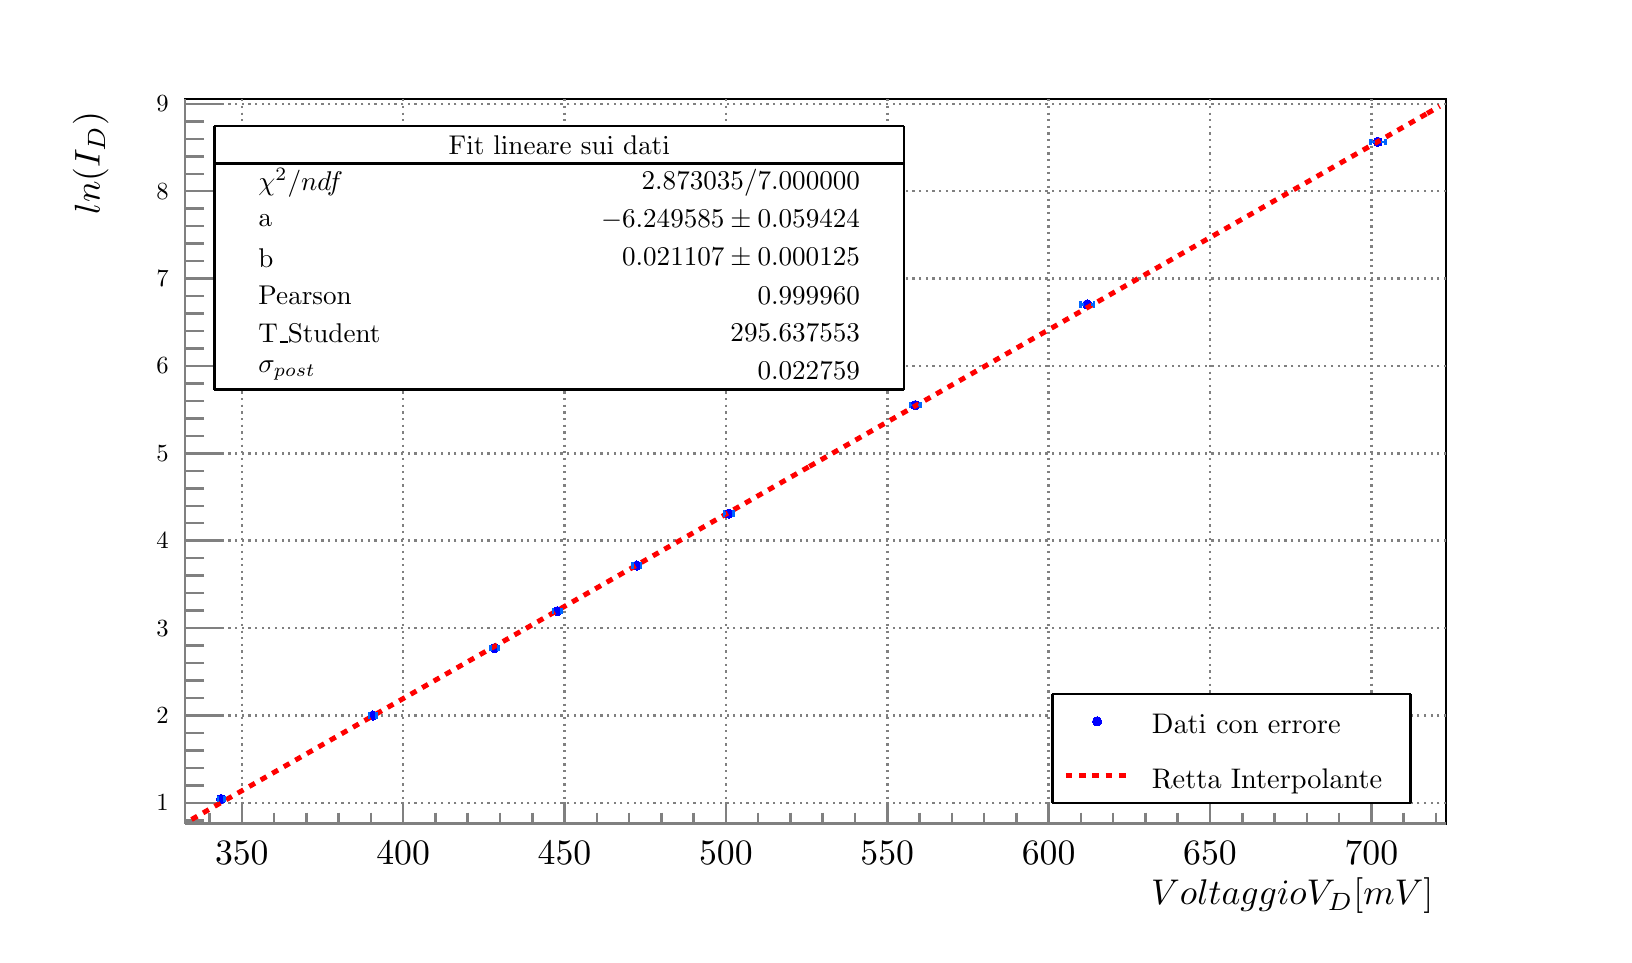
\begin{tikzpicture}
\pgfdeclareplotmark{cross} {
\pgfpathmoveto{\pgfpoint{-0.3\pgfplotmarksize}{\pgfplotmarksize}}
\pgfpathlineto{\pgfpoint{+0.3\pgfplotmarksize}{\pgfplotmarksize}}
\pgfpathlineto{\pgfpoint{+0.3\pgfplotmarksize}{0.3\pgfplotmarksize}}
\pgfpathlineto{\pgfpoint{+1\pgfplotmarksize}{0.3\pgfplotmarksize}}
\pgfpathlineto{\pgfpoint{+1\pgfplotmarksize}{-0.3\pgfplotmarksize}}
\pgfpathlineto{\pgfpoint{+0.3\pgfplotmarksize}{-0.3\pgfplotmarksize}}
\pgfpathlineto{\pgfpoint{+0.3\pgfplotmarksize}{-1.\pgfplotmarksize}}
\pgfpathlineto{\pgfpoint{-0.3\pgfplotmarksize}{-1.\pgfplotmarksize}}
\pgfpathlineto{\pgfpoint{-0.3\pgfplotmarksize}{-0.3\pgfplotmarksize}}
\pgfpathlineto{\pgfpoint{-1.\pgfplotmarksize}{-0.3\pgfplotmarksize}}
\pgfpathlineto{\pgfpoint{-1.\pgfplotmarksize}{0.3\pgfplotmarksize}}
\pgfpathlineto{\pgfpoint{-0.3\pgfplotmarksize}{0.3\pgfplotmarksize}}
\pgfpathclose
\pgfusepathqstroke
}
\pgfdeclareplotmark{cross*} {
\pgfpathmoveto{\pgfpoint{-0.3\pgfplotmarksize}{\pgfplotmarksize}}
\pgfpathlineto{\pgfpoint{+0.3\pgfplotmarksize}{\pgfplotmarksize}}
\pgfpathlineto{\pgfpoint{+0.3\pgfplotmarksize}{0.3\pgfplotmarksize}}
\pgfpathlineto{\pgfpoint{+1\pgfplotmarksize}{0.3\pgfplotmarksize}}
\pgfpathlineto{\pgfpoint{+1\pgfplotmarksize}{-0.3\pgfplotmarksize}}
\pgfpathlineto{\pgfpoint{+0.3\pgfplotmarksize}{-0.3\pgfplotmarksize}}
\pgfpathlineto{\pgfpoint{+0.3\pgfplotmarksize}{-1.\pgfplotmarksize}}
\pgfpathlineto{\pgfpoint{-0.3\pgfplotmarksize}{-1.\pgfplotmarksize}}
\pgfpathlineto{\pgfpoint{-0.3\pgfplotmarksize}{-0.3\pgfplotmarksize}}
\pgfpathlineto{\pgfpoint{-1.\pgfplotmarksize}{-0.3\pgfplotmarksize}}
\pgfpathlineto{\pgfpoint{-1.\pgfplotmarksize}{0.3\pgfplotmarksize}}
\pgfpathlineto{\pgfpoint{-0.3\pgfplotmarksize}{0.3\pgfplotmarksize}}
\pgfpathclose
\pgfusepathqfillstroke
}
\pgfdeclareplotmark{newstar} {
\pgfpathmoveto{\pgfqpoint{0pt}{\pgfplotmarksize}}
\pgfpathlineto{\pgfqpointpolar{44}{0.5\pgfplotmarksize}}
\pgfpathlineto{\pgfqpointpolar{18}{\pgfplotmarksize}}
\pgfpathlineto{\pgfqpointpolar{-20}{0.5\pgfplotmarksize}}
\pgfpathlineto{\pgfqpointpolar{-54}{\pgfplotmarksize}}
\pgfpathlineto{\pgfqpointpolar{-90}{0.5\pgfplotmarksize}}
\pgfpathlineto{\pgfqpointpolar{234}{\pgfplotmarksize}}
\pgfpathlineto{\pgfqpointpolar{198}{0.5\pgfplotmarksize}}
\pgfpathlineto{\pgfqpointpolar{162}{\pgfplotmarksize}}
\pgfpathlineto{\pgfqpointpolar{134}{0.5\pgfplotmarksize}}
\pgfpathclose
\pgfusepathqstroke
}
\pgfdeclareplotmark{newstar*} {
\pgfpathmoveto{\pgfqpoint{0pt}{\pgfplotmarksize}}
\pgfpathlineto{\pgfqpointpolar{44}{0.5\pgfplotmarksize}}
\pgfpathlineto{\pgfqpointpolar{18}{\pgfplotmarksize}}
\pgfpathlineto{\pgfqpointpolar{-20}{0.5\pgfplotmarksize}}
\pgfpathlineto{\pgfqpointpolar{-54}{\pgfplotmarksize}}
\pgfpathlineto{\pgfqpointpolar{-90}{0.5\pgfplotmarksize}}
\pgfpathlineto{\pgfqpointpolar{234}{\pgfplotmarksize}}
\pgfpathlineto{\pgfqpointpolar{198}{0.5\pgfplotmarksize}}
\pgfpathlineto{\pgfqpointpolar{162}{\pgfplotmarksize}}
\pgfpathlineto{\pgfqpointpolar{134}{0.5\pgfplotmarksize}}
\pgfpathclose
\pgfusepathqfillstroke
}
\definecolor{c}{rgb}{1,1,1};
\draw [color=c, fill=c] (0,0) rectangle (20,11.503);
\draw [color=c, fill=c] (1.99399,1.40281) rectangle (18.006,10.6012);
\definecolor{c}{rgb}{0,0,0};
\draw [c,line width=0.9] (1.99399,1.40281) -- (1.99399,10.6012) -- (18.006,10.6012) -- (18.006,1.40281) -- (1.99399,1.40281);
\definecolor{c}{rgb}{1,1,1};
\draw [color=c, fill=c] (1.99399,1.40281) rectangle (18.006,10.6012);
\definecolor{c}{rgb}{0,0,0};
\draw [c,line width=0.9] (1.99399,1.40281) -- (1.99399,10.6012) -- (18.006,10.6012) -- (18.006,1.40281) -- (1.99399,1.40281);
\definecolor{c}{rgb}{0.5,0.5,0.5};
\draw [c,line width=0.9] (1.99399,1.40281) -- (18.006,1.40281);
\draw [c,dash pattern=on 0.80pt off 1.60pt ,line width=0.9] (2.71235,10.6012) -- (2.71235,1.40281);
\draw [c,dash pattern=on 0.80pt off 1.60pt ,line width=0.9] (4.76166,10.6012) -- (4.76166,1.40281);
\draw [c,dash pattern=on 0.80pt off 1.60pt ,line width=0.9] (6.81097,10.6012) -- (6.81097,1.40281);
\draw [c,dash pattern=on 0.80pt off 1.60pt ,line width=0.9] (8.86027,10.6012) -- (8.86027,1.40281);
\draw [c,dash pattern=on 0.80pt off 1.60pt ,line width=0.9] (10.9096,10.6012) -- (10.9096,1.40281);
\draw [c,dash pattern=on 0.80pt off 1.60pt ,line width=0.9] (12.9589,10.6012) -- (12.9589,1.40281);
\draw [c,dash pattern=on 0.80pt off 1.60pt ,line width=0.9] (15.0082,10.6012) -- (15.0082,1.40281);
\draw [c,dash pattern=on 0.80pt off 1.60pt ,line width=0.9] (17.0575,10.6012) -- (17.0575,1.40281);
\draw [c,dash pattern=on 0.80pt off 1.60pt ,line width=0.9] (2.71235,10.6012) -- (2.71235,1.40281);
\draw [c,dash pattern=on 0.80pt off 1.60pt ,line width=0.9] (17.0575,10.6012) -- (17.0575,1.40281);
\draw [c,line width=0.9] (1.99399,1.40281) -- (1.99399,10.6012);
\draw [c,dash pattern=on 0.80pt off 1.60pt ,line width=0.9] (18.006,1.66546) -- (1.99399,1.66546);
\draw [c,dash pattern=on 0.80pt off 1.60pt ,line width=0.9] (18.006,2.77503) -- (1.99399,2.77503);
\draw [c,dash pattern=on 0.80pt off 1.60pt ,line width=0.9] (18.006,3.8846) -- (1.99399,3.8846);
\draw [c,dash pattern=on 0.80pt off 1.60pt ,line width=0.9] (18.006,4.99417) -- (1.99399,4.99417);
\draw [c,dash pattern=on 0.80pt off 1.60pt ,line width=0.9] (18.006,6.10375) -- (1.99399,6.10375);
\draw [c,dash pattern=on 0.80pt off 1.60pt ,line width=0.9] (18.006,7.21332) -- (1.99399,7.21332);
\draw [c,dash pattern=on 0.80pt off 1.60pt ,line width=0.9] (18.006,8.32289) -- (1.99399,8.32289);
\draw [c,dash pattern=on 0.80pt off 1.60pt ,line width=0.9] (18.006,9.43247) -- (1.99399,9.43247);
\draw [c,dash pattern=on 0.80pt off 1.60pt ,line width=0.9] (18.006,10.542) -- (1.99399,10.542);
\draw [c,dash pattern=on 0.80pt off 1.60pt ,line width=0.9] (18.006,1.66546) -- (1.99399,1.66546);
\draw [c,dash pattern=on 0.80pt off 1.60pt ,line width=0.9] (18.006,10.542) -- (1.99399,10.542);
\draw [c,line width=0.9] (1.99399,1.40281) -- (18.006,1.40281);
\draw [c,line width=0.9] (2.71235,1.67909) -- (2.71235,1.40281);
\draw [c,line width=0.9] (3.12221,1.54095) -- (3.12221,1.40281);
\draw [c,line width=0.9] (3.53208,1.54095) -- (3.53208,1.40281);
\draw [c,line width=0.9] (3.94194,1.54095) -- (3.94194,1.40281);
\draw [c,line width=0.9] (4.3518,1.54095) -- (4.3518,1.40281);
\draw [c,line width=0.9] (4.76166,1.67909) -- (4.76166,1.40281);
\draw [c,line width=0.9] (5.17152,1.54095) -- (5.17152,1.40281);
\draw [c,line width=0.9] (5.58138,1.54095) -- (5.58138,1.40281);
\draw [c,line width=0.9] (5.99124,1.54095) -- (5.99124,1.40281);
\draw [c,line width=0.9] (6.4011,1.54095) -- (6.4011,1.40281);
\draw [c,line width=0.9] (6.81097,1.67909) -- (6.81097,1.40281);
\draw [c,line width=0.9] (7.22083,1.54095) -- (7.22083,1.40281);
\draw [c,line width=0.9] (7.63069,1.54095) -- (7.63069,1.40281);
\draw [c,line width=0.9] (8.04055,1.54095) -- (8.04055,1.40281);
\draw [c,line width=0.9] (8.45041,1.54095) -- (8.45041,1.40281);
\draw [c,line width=0.9] (8.86027,1.67909) -- (8.86027,1.40281);
\draw [c,line width=0.9] (9.27013,1.54095) -- (9.27013,1.40281);
\draw [c,line width=0.9] (9.67999,1.54095) -- (9.67999,1.40281);
\draw [c,line width=0.9] (10.0899,1.54095) -- (10.0899,1.40281);
\draw [c,line width=0.9] (10.4997,1.54095) -- (10.4997,1.40281);
\draw [c,line width=0.9] (10.9096,1.67909) -- (10.9096,1.40281);
\draw [c,line width=0.9] (11.3194,1.54095) -- (11.3194,1.40281);
\draw [c,line width=0.9] (11.7293,1.54095) -- (11.7293,1.40281);
\draw [c,line width=0.9] (12.1392,1.54095) -- (12.1392,1.40281);
\draw [c,line width=0.9] (12.549,1.54095) -- (12.549,1.40281);
\draw [c,line width=0.9] (12.9589,1.67909) -- (12.9589,1.40281);
\draw [c,line width=0.9] (13.3687,1.54095) -- (13.3687,1.40281);
\draw [c,line width=0.9] (13.7786,1.54095) -- (13.7786,1.40281);
\draw [c,line width=0.9] (14.1885,1.54095) -- (14.1885,1.40281);
\draw [c,line width=0.9] (14.5983,1.54095) -- (14.5983,1.40281);
\draw [c,line width=0.9] (15.0082,1.67909) -- (15.0082,1.40281);
\draw [c,line width=0.9] (15.4181,1.54095) -- (15.4181,1.40281);
\draw [c,line width=0.9] (15.8279,1.54095) -- (15.8279,1.40281);
\draw [c,line width=0.9] (16.2378,1.54095) -- (16.2378,1.40281);
\draw [c,line width=0.9] (16.6476,1.54095) -- (16.6476,1.40281);
\draw [c,line width=0.9] (17.0575,1.67909) -- (17.0575,1.40281);
\draw [c,line width=0.9] (2.71235,1.67909) -- (2.71235,1.40281);
\draw [c,line width=0.9] (2.30249,1.54095) -- (2.30249,1.40281);
\draw [c,line width=0.9] (17.0575,1.67909) -- (17.0575,1.40281);
\draw [c,line width=0.9] (17.4674,1.54095) -- (17.4674,1.40281);
\draw [c,line width=0.9] (17.8772,1.54095) -- (17.8772,1.40281);
\definecolor{c}{rgb}{0,0,0};
\draw [anchor=base] (2.71235,0.88517) node[scale=1.29074, color=c, rotate=0]{350};
\draw [anchor=base] (4.76166,0.88517) node[scale=1.29074, color=c, rotate=0]{400};
\draw [anchor=base] (6.81097,0.88517) node[scale=1.29074, color=c, rotate=0]{450};
\draw [anchor=base] (8.86027,0.88517) node[scale=1.29074, color=c, rotate=0]{500};
\draw [anchor=base] (10.9096,0.88517) node[scale=1.29074, color=c, rotate=0]{550};
\draw [anchor=base] (12.9589,0.88517) node[scale=1.29074, color=c, rotate=0]{600};
\draw [anchor=base] (15.0082,0.88517) node[scale=1.29074, color=c, rotate=0]{650};
\draw [anchor=base] (17.0575,0.88517) node[scale=1.29074, color=c, rotate=0]{700};
\draw [anchor= east] (18.006,0.482565) node[scale=1.29074, color=c, rotate=0]{$Voltaggio V_{D} [mV]$};
\definecolor{c}{rgb}{0.5,0.5,0.5};
\draw [c,line width=0.9] (1.99399,1.40281) -- (1.99399,10.6012);
\draw [c,line width=0.9] (2.47378,1.66546) -- (1.99399,1.66546);
\draw [c,line width=0.9] (2.23388,1.88737) -- (1.99399,1.88737);
\draw [c,line width=0.9] (2.23388,2.10928) -- (1.99399,2.10928);
\draw [c,line width=0.9] (2.23388,2.3312) -- (1.99399,2.3312);
\draw [c,line width=0.9] (2.23388,2.55311) -- (1.99399,2.55311);
\draw [c,line width=0.9] (2.47378,2.77503) -- (1.99399,2.77503);
\draw [c,line width=0.9] (2.23388,2.99694) -- (1.99399,2.99694);
\draw [c,line width=0.9] (2.23388,3.21886) -- (1.99399,3.21886);
\draw [c,line width=0.9] (2.23388,3.44077) -- (1.99399,3.44077);
\draw [c,line width=0.9] (2.23388,3.66269) -- (1.99399,3.66269);
\draw [c,line width=0.9] (2.47378,3.8846) -- (1.99399,3.8846);
\draw [c,line width=0.9] (2.23388,4.10652) -- (1.99399,4.10652);
\draw [c,line width=0.9] (2.23388,4.32843) -- (1.99399,4.32843);
\draw [c,line width=0.9] (2.23388,4.55034) -- (1.99399,4.55034);
\draw [c,line width=0.9] (2.23388,4.77226) -- (1.99399,4.77226);
\draw [c,line width=0.9] (2.47378,4.99417) -- (1.99399,4.99417);
\draw [c,line width=0.9] (2.23388,5.21609) -- (1.99399,5.21609);
\draw [c,line width=0.9] (2.23388,5.438) -- (1.99399,5.438);
\draw [c,line width=0.9] (2.23388,5.65992) -- (1.99399,5.65992);
\draw [c,line width=0.9] (2.23388,5.88183) -- (1.99399,5.88183);
\draw [c,line width=0.9] (2.47378,6.10375) -- (1.99399,6.10375);
\draw [c,line width=0.9] (2.23388,6.32566) -- (1.99399,6.32566);
\draw [c,line width=0.9] (2.23388,6.54758) -- (1.99399,6.54758);
\draw [c,line width=0.9] (2.23388,6.76949) -- (1.99399,6.76949);
\draw [c,line width=0.9] (2.23388,6.99141) -- (1.99399,6.99141);
\draw [c,line width=0.9] (2.47378,7.21332) -- (1.99399,7.21332);
\draw [c,line width=0.9] (2.23388,7.43524) -- (1.99399,7.43524);
\draw [c,line width=0.9] (2.23388,7.65715) -- (1.99399,7.65715);
\draw [c,line width=0.9] (2.23388,7.87906) -- (1.99399,7.87906);
\draw [c,line width=0.9] (2.23388,8.10098) -- (1.99399,8.10098);
\draw [c,line width=0.9] (2.47378,8.32289) -- (1.99399,8.32289);
\draw [c,line width=0.9] (2.23388,8.54481) -- (1.99399,8.54481);
\draw [c,line width=0.9] (2.23388,8.76672) -- (1.99399,8.76672);
\draw [c,line width=0.9] (2.23388,8.98864) -- (1.99399,8.98864);
\draw [c,line width=0.9] (2.23388,9.21055) -- (1.99399,9.21055);
\draw [c,line width=0.9] (2.47378,9.43247) -- (1.99399,9.43247);
\draw [c,line width=0.9] (2.23388,9.65438) -- (1.99399,9.65438);
\draw [c,line width=0.9] (2.23388,9.8763) -- (1.99399,9.8763);
\draw [c,line width=0.9] (2.23388,10.0982) -- (1.99399,10.0982);
\draw [c,line width=0.9] (2.23388,10.3201) -- (1.99399,10.3201);
\draw [c,line width=0.9] (2.47378,10.542) -- (1.99399,10.542);
\draw [c,line width=0.9] (2.47378,1.66546) -- (1.99399,1.66546);
\draw [c,line width=0.9] (2.23388,1.44354) -- (1.99399,1.44354);
\draw [c,line width=0.9] (2.47378,10.542) -- (1.99399,10.542);
\definecolor{c}{rgb}{0,0,0};
\draw [anchor= east] (1.89399,1.66546) node[scale=0.890168, color=c, rotate=0]{1};
\draw [anchor= east] (1.89399,2.77503) node[scale=0.890168, color=c, rotate=0]{2};
\draw [anchor= east] (1.89399,3.8846) node[scale=0.890168, color=c, rotate=0]{3};
\draw [anchor= east] (1.89399,4.99417) node[scale=0.890168, color=c, rotate=0]{4};
\draw [anchor= east] (1.89399,6.10375) node[scale=0.890168, color=c, rotate=0]{5};
\draw [anchor= east] (1.89399,7.21332) node[scale=0.890168, color=c, rotate=0]{6};
\draw [anchor= east] (1.89399,8.32289) node[scale=0.890168, color=c, rotate=0]{7};
\draw [anchor= east] (1.89399,9.43247) node[scale=0.890168, color=c, rotate=0]{8};
\draw [anchor= east] (1.89399,10.542) node[scale=0.890168, color=c, rotate=0]{9};
\draw [anchor= east] (0.793587,10.6012) node[scale=1.29074, color=c, rotate=90]{$ln(I_{D}) $};
\definecolor{c}{rgb}{0,0,1};
\foreach \P in {(2.45004,1.71406), (4.37639,2.77367), (5.92157,3.63019), (6.7208,4.0996), (7.72905,4.67852), (8.89716,5.33799), (11.2662,6.71613), (13.4507,7.99557), (17.1395,10.0605)}{\draw[mark options={color=c,fill=c},mark size=1.681682pt, line
 width=0.000000pt, mark=*] plot coordinates {\P};}
\definecolor{c}{rgb}{1,0,0};
\draw [c,dash pattern=on 2.40pt off 2.40pt ,line width=1.8] (2.07405,1.45385) -- (2.23417,1.54534) -- (2.39429,1.63684) -- (2.55441,1.72833) -- (2.71453,1.81983) -- (2.87465,1.91133) -- (3.03477,2.00282) -- (3.19489,2.09432) -- (3.35501,2.18581) --
 (3.51513,2.27731) -- (3.67525,2.3688) -- (3.83537,2.4603) -- (3.99549,2.5518) -- (4.15561,2.64329) -- (4.31573,2.73479) -- (4.47585,2.82628) -- (4.63597,2.91778) -- (4.79609,3.00927) -- (4.95621,3.10077) -- (5.11633,3.19227) -- (5.27645,3.28376) --
 (5.43657,3.37526) -- (5.59669,3.46675) -- (5.75681,3.55825) -- (5.91693,3.64974) -- (6.07705,3.74124) -- (6.23717,3.83273) -- (6.39729,3.92423) -- (6.55741,4.01573) -- (6.71754,4.10722) -- (6.87766,4.19872) -- (7.03778,4.29021) -- (7.1979,4.38171)
 -- (7.35802,4.4732) -- (7.51814,4.5647) -- (7.67826,4.6562) -- (7.83838,4.74769) -- (7.9985,4.83919) -- (8.15862,4.93068) -- (8.31874,5.02218) -- (8.47886,5.11367) -- (8.63898,5.20517) -- (8.7991,5.29667) -- (8.95922,5.38816) -- (9.11934,5.47966) --
 (9.27946,5.57115) -- (9.43958,5.66265) -- (9.5997,5.75414) -- (9.75982,5.84564) -- (9.91994,5.93713);
\draw [c,dash pattern=on 2.40pt off 2.40pt ,line width=1.8] (9.91994,5.93713) -- (10.0801,6.02863) -- (10.2402,6.12013) -- (10.4003,6.21162) -- (10.5604,6.30312) -- (10.7205,6.39461) -- (10.8807,6.48611) -- (11.0408,6.5776) -- (11.2009,6.6691) --
 (11.361,6.7606) -- (11.5211,6.85209) -- (11.6813,6.94359) -- (11.8414,7.03508) -- (12.0015,7.12658) -- (12.1616,7.21807) -- (12.3217,7.30957) -- (12.4819,7.40106) -- (12.642,7.49256) -- (12.8021,7.58406) -- (12.9622,7.67555) -- (13.1223,7.76705) --
 (13.2825,7.85854) -- (13.4426,7.95004) -- (13.6027,8.04153) -- (13.7628,8.13303) -- (13.9229,8.22453) -- (14.0831,8.31602) -- (14.2432,8.40752) -- (14.4033,8.49901) -- (14.5634,8.59051) -- (14.7235,8.682) -- (14.8837,8.7735) -- (15.0438,8.865) --
 (15.2039,8.95649) -- (15.364,9.04799) -- (15.5241,9.13948) -- (15.6843,9.23098) -- (15.8444,9.32247) -- (16.0045,9.41397) -- (16.1646,9.50546) -- (16.3247,9.59696) -- (16.4849,9.68846) -- (16.645,9.77995) -- (16.8051,9.87145) -- (16.9652,9.96294) --
 (17.1254,10.0544) -- (17.2855,10.1459) -- (17.4456,10.2374) -- (17.6057,10.3289) -- (17.7658,10.4204);
\draw [c,dash pattern=on 2.40pt off 2.40pt ,line width=1.8] (17.7658,10.4204) -- (17.926,10.5119);
\definecolor{c}{rgb}{0,0.4,1};
\draw [c,line width=0.9] (2.40996,1.71406) -- (2.40911,1.71406);
\draw [c,line width=0.9] (2.40911,1.67398) -- (2.40911,1.75414);
\draw [c,line width=0.9] (2.49012,1.71406) -- (2.49097,1.71406);
\draw [c,line width=0.9] (2.49097,1.67398) -- (2.49097,1.75414);
\draw [c,line width=0.9] (4.33631,2.77367) -- (4.32993,2.77367);
\draw [c,line width=0.9] (4.32993,2.73359) -- (4.32993,2.81375);
\draw [c,line width=0.9] (4.41647,2.77367) -- (4.42285,2.77367);
\draw [c,line width=0.9] (4.42285,2.73359) -- (4.42285,2.81375);
\draw [c,line width=0.9] (5.88149,3.63019) -- (5.87067,3.63019);
\draw [c,line width=0.9] (5.87067,3.59011) -- (5.87067,3.67027);
\draw [c,line width=0.9] (5.96165,3.63019) -- (5.97246,3.63019);
\draw [c,line width=0.9] (5.97246,3.59011) -- (5.97246,3.67027);
\draw [c,line width=0.9] (6.68072,4.0996) -- (6.6676,4.0996);
\draw [c,line width=0.9] (6.6676,4.05952) -- (6.6676,4.13968);
\draw [c,line width=0.9] (6.76088,4.0996) -- (6.77399,4.0996);
\draw [c,line width=0.9] (6.77399,4.05952) -- (6.77399,4.13968);
\draw [c,line width=0.9] (7.68897,4.67852) -- (7.67296,4.67852);
\draw [c,line width=0.9] (7.67296,4.63844) -- (7.67296,4.7186);
\draw [c,line width=0.9] (7.76913,4.67852) -- (7.78515,4.67852);
\draw [c,line width=0.9] (7.78515,4.63844) -- (7.78515,4.7186);
\draw [c,line width=0.9] (8.85708,5.33799) -- (8.83771,5.33799);
\draw [c,line width=0.9] (8.83771,5.29791) -- (8.83771,5.37807);
\draw [c,line width=0.9] (8.93724,5.33799) -- (8.95661,5.33799);
\draw [c,line width=0.9] (8.95661,5.29791) -- (8.95661,5.37807);
\draw [c,line width=0.9] (11.2261,6.71613) -- (11.1999,6.71613);
\draw [c,line width=0.9] (11.1999,6.67605) -- (11.1999,6.75621);
\draw [c,line width=0.9] (11.3062,6.71613) -- (11.3324,6.71613);
\draw [c,line width=0.9] (11.3324,6.67605) -- (11.3324,6.75621);
\draw [c,line width=0.9] (13.4106,7.99557) -- (13.3642,7.99557);
\draw [c,line width=0.9] (13.3642,7.95549) -- (13.3642,8.03565);
\draw [c,line width=0.9] (13.4908,7.99557) -- (13.5372,7.99557);
\draw [c,line width=0.9] (13.5372,7.95549) -- (13.5372,8.03565);
\draw [c,line width=0.9] (17.0994,10.0605) -- (17.0439,10.0605);
\draw [c,line width=0.9] (17.0439,10.0204) -- (17.0439,10.1005);
\draw [c,line width=0.9] (17.1795,10.0605) -- (17.2351,10.0605);
\draw [c,line width=0.9] (17.2351,10.0204) -- (17.2351,10.1005);
\definecolor{c}{rgb}{1,1,1};
\draw [color=c, fill=c] (2.36473,6.91383) rectangle (11.1222,10.2605);
\definecolor{c}{rgb}{0,0,0};
\draw [c,line width=0.9] (2.36473,6.91383) -- (11.1222,6.91383);
\draw [c,line width=0.9] (11.1222,6.91383) -- (11.1222,10.2605);
\draw [c,line width=0.9] (11.1222,10.2605) -- (2.36473,10.2605);
\draw [c,line width=0.9] (2.36473,10.2605) -- (2.36473,6.91383);
\draw (6.74349,10.0215) node[scale=0.979185, color=c, rotate=0]{Fit lineare sui dati};
\draw [c,line width=0.9] (2.36473,9.78242) -- (11.1222,9.78242);
\draw [anchor= west] (2.80261,9.54337) node[scale=0.979185, color=c, rotate=0]{$\chi^{2} / ndf $};
\draw [anchor= east] (10.6844,9.54337) node[scale=0.979185, color=c, rotate=0]{2.873035/7.000000};
\draw [anchor= west] (2.80261,9.06527) node[scale=0.979185, color=c, rotate=0]{a        };
\draw [anchor= east] (10.6844,9.06527) node[scale=0.979185, color=c, rotate=0]{$ -6.249585\pm0.059424$};
\draw [anchor= west] (2.80261,8.58717) node[scale=0.979185, color=c, rotate=0]{b        };
\draw [anchor= east] (10.6844,8.58717) node[scale=0.979185, color=c, rotate=0]{$ 0.021107\pm0.000125$};
\draw [anchor= west] (2.80261,8.10908) node[scale=0.979185, color=c, rotate=0]{Pearson        };
\draw [anchor= east] (10.6844,8.10908) node[scale=0.979185, color=c, rotate=0]{ 0.999960};
\draw [anchor= west] (2.80261,7.63098) node[scale=0.979185, color=c, rotate=0]{T\_Student        };
\draw [anchor= east] (10.6844,7.63098) node[scale=0.979185, color=c, rotate=0]{ 295.637553};
\draw [anchor= west] (2.80261,7.15288) node[scale=0.979185, color=c, rotate=0]{$\sigma_{post}        $};
\draw [anchor= east] (10.6844,7.15288) node[scale=0.979185, color=c, rotate=0]{ 0.022759};
\definecolor{c}{rgb}{1,1,1};
\draw [color=c, fill=c] (13.006,1.66333) rectangle (17.5551,3.04609);
\definecolor{c}{rgb}{0,0,0};
\draw [c,line width=0.9] (13.006,1.66333) -- (17.5551,1.66333);
\draw [c,line width=0.9] (17.5551,1.66333) -- (17.5551,3.04609);
\draw [c,line width=0.9] (17.5551,3.04609) -- (13.006,3.04609);
\draw [c,line width=0.9] (13.006,3.04609) -- (13.006,1.66333);
\draw [anchor=base west] (14.1433,2.54484) node[scale=1.02369, color=c, rotate=0]{Dati con errore};
\definecolor{c}{rgb}{0,0,1};
\foreach \P in {(13.5746,2.7004)}{\draw[mark options={color=c,fill=c},mark size=1.681682pt, line width=0.000000pt, mark=*] plot coordinates {\P};}
\definecolor{c}{rgb}{0,0,0};
\draw [anchor=base west] (14.1433,1.85346) node[scale=1.02369, color=c, rotate=0]{Retta Interpolante};
\definecolor{c}{rgb}{1,0,0};
\draw [c,dash pattern=on 2.40pt off 2.40pt ,line width=1.8] (13.1766,2.00902) -- (13.9727,2.00902);
\end{tikzpicture}
